\chapter{Logistik}
\label{chap:Logistik}

Laut einer Bitkom-Studie aus dem aktuellen Jahr sehen 92 \% der befragten Logistikunternehmen eine Beschleunigung im Transport von Produkten mithilfe der Digitalisierung gegeben \cite{Bitkom2019}. Generell ist in der Branche zunehmen ein Drang nach Digitalisierung aufgrund der komplexen Prozessketten zu sehen. Wo in der Logistik Abmachungen zwischen Vertragsteilnehmern stattfinden, lassen sich Systeme auch ideal mittels Smart Contracts umsetzen. 

\section{Dachser}
Im Vorlauf zu dieser Arbeit und der dazugehörigen Präsentation konnte eine Besprechung mit einem fachkundigen Mitarbeiter der Firma Dachser aus Kempten durchgeführt werden. Seit 2016 wird dort in Zusammenarbeit mit dem Fraunhofer Institut an der Sinnhaftigkeit von Blockchain-Anwendungen sowie Smart Contracts und deren Use Cases geforscht. Dabei werden besonders zwei mögliche Systeme in Betracht gezogen: Hyperledger und Ethereum. Ziel ist es, die Technologie hinter den bekannt gewordenen Schlagworten zu verstehen.

\begin{figure}[h!]
  \centering
  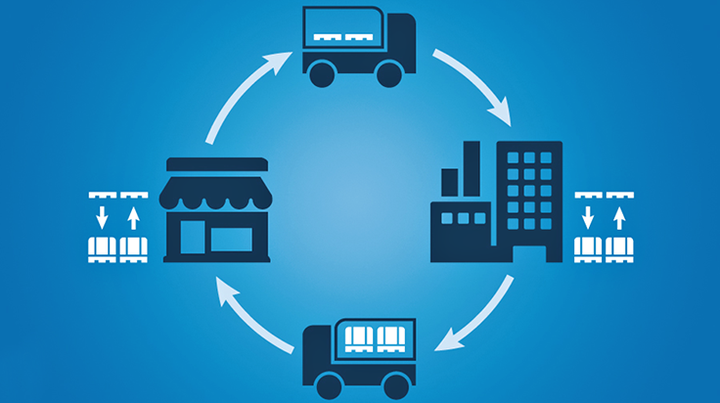
\includegraphics[width=\textwidth]{Bilder/Palettentausch.png}
  \caption[Palettentausch]{Palettentausch \cite{Disponaut2016}}
  \label{fig:palettentausch}
\end{figure}

Ein konkreter Anwendungsfall wurde im Rahmen einer Bachelorarbeit im Wintersemester 2018/2019 prototypisch umgesetzt. Dabei wurde exemplarisch der Palettentausch herangezogen. Diese Aufgabe stellt eine höhere organisatorische Hürde da als man anfangs vermuten würde. Betrachtet man das einfache Beispiel aus Abbildung \ref{fig:palettentausch}, sieht man einen immer wiederkehrenden Kreislauf. Sinn und Zweck des Palettentausch ist es, immer eins zu eins vollständig leere Europaletten gegen mit Ware beladene zu wechseln. Deshalb muss der Lastkraftwagen zunächst mit leeren Paletten beladen zum Produzenten fahren um dort die Ware zu beladen, welche er sodann zum Kunden transportiert. Dort angekommen erhält er wieder in gleicher Anzahl zur Lieferung leere Paletten. In der Praxis stellt sich das jedoch nicht als realistisches Szenario dar: Bei voller Beladung mit leeren Paletten muss immer noch genügend Platz für unpalettierte Ware vorhanden sein. Dadurch ist ein gleichmäßiger Palettentausch nicht durchsetzbar. Mittels oft nicht standardisierten Papierformularen, sogenannten Palettenscheinen, wird der Austausch zwischen den Geschäftspartnern quittiert. Sollte es zu einer ungleichmäßigen Verteilung kommen, wird ein Kontenbetrag von jedem Teilnehmer selbstständig abgebucht, um einen Ausgleich herzustellen. \cite[vgl.][]{Disponaut2016}

In der Zwischenzeit gab es eine Initiative der GS1, um den Palettenschein zu standardisieren und digitalisieren \cite[vgl.][]{GS12017}. Dadurch soll es auch möglich sein, ihn elektronisch untereinander auszutauschen. Ein Problem aber bleibt; die eigenhändige Abrechnung der beiden Parteien. Hier offenbart sich ein entscheidender Vorteil eines Smart Contracts. Da er die Kontostände der Teilnehmer kennt, kann er an zentraler Stelle die Schulden auf die jeweiligen Konten buchen. Dadurch fällt ein großer Teil der organisatorischen Komplexität weg. So wurde es auch in einem Proof of Concept in der oben genannten Bachelorthesis gezeigt, welcher aber nie im Produktionsmodus angewandt wurde.

Allgemein hat sich bei der Firma Dachser herausgestellt, dass die Blockchain und die darunterliegenden Smart Contracts nicht unter den aktuellen Gegebenheiten als sinnbringende Technologien eingesetzt werden können. Damit es eine praktikable Lösung darstellt, müssten weitere Industriepartner in die Blockchain eingebunden werden, darunter auch direkte Konkurrenten der Firma Dachser, wie beispielsweise DB Schenker. Per Definition kann nun jeder die Transaktionen, welche bei einem Smart Contract anfallen, nachvollziehen. Wollte man die Sichtbarkeit untereinander einschränken, müsste man die Blockchain so abändern, dass sie im Endeffekt nicht mehr ihrer eigentlichen Bestimmung gerecht wird. In der Branche wird ein Umdenken gefordert, damit nützliche Modelle nicht an der Umsetzung scheitern müssen. Letztendlich hängt ein Großteil nicht an der Technik, sondern an der unternehmenspolitischen Ausführung.\\
Ein weiteres Manko ist das Fehlen von Standards bei der Implementierung von Smart Contracts, da sie nicht im Nachhinein vom Programmierer abgeändert werden können. Das sorgt zusehends für Verwirrung und Ungereimtheiten bei der Implementierung, was bei klassischen Systemen durch Industrie- und Programmierstandards nahezu ausgeschlossen werden kann. Oftmals stellt sich eine herkömmliche Lösung als einfacher und tragfähiger heraus, besonders dort, wo sowieso nur ein Server/Node benötigt wird, was die dezentrale Implementierung in einer Blockchain obsolet macht.\\
Betrachtet man die heutigen Anforderungen an den Datenschutz im Unternehmen, so steht die Speicherung in einer Blockchain unter Umständen in klarem Kontrast du den Forderungen der Datenschutzgrundverordnung. Diese fordert eine Löschbarkeit bzw. Anonymisierung der Daten bei Erstellung respektive im Nachhinein. Durch die Unveränderlichkeit der Blockchain ist das schlichtweg nicht durchführbar. Die aktuell vorherrschenden Gesetze bieten keine Möglichkeit, Probleme wie den Palettentausch mit Palettenschein sinnvoll auf einen Smart Contract abzubilden.

\section{Tradelens}
Eine erfolgreich im Markt bestehende Softwarelösung ist Tradelens, ein Produkt, welches in Kooperation von IBM und der dänischen Reederei Maersk entstanden ist. Das Ziel ist, eine Plattform für möglichst viele Beteiligte zu liefern, um damit an der Spitze der digitalen Transformation in der Logistik zu stehen \cite[vgl.][S. 7]{Tradelens2019b}. Tradelens besteht aus insgesamt drei Ebenen: Netzwerk, Plattform und Applikationen (siehe Abbildung \ref{fig:tradelensOverview}).

\begin{figure}[h!]
  \centering
  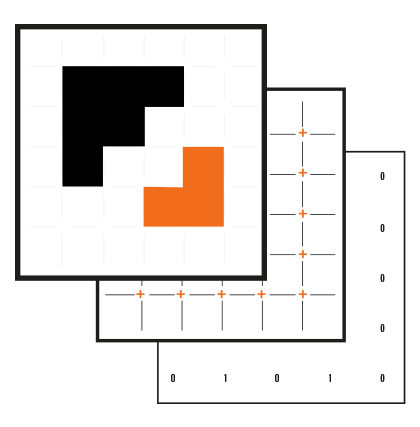
\includegraphics[width=.4\textwidth]{Bilder/Tradelens-Overview.png}
  \caption[Tradelens Aufbau]{Tradelens Aufbau \cite{Tradelens2019a}}
  \label{fig:tradelensOverview}
\end{figure}

\textbf{Netzwerk}\\
Das Netzwerk bildet die Grundlage von Tradelens. Formal beschrieben umfasst es alle Business-Teilnehmer, welche an dieser spezifischen Blockchain-Lösung teilnehmen. So ist es möglich, die Teilhabenden an der gesamten Supply-Chain abzudecken. Dies reicht von den Verschiffern, über Versandunternehmer bis zu Regierung und das zuständigen Zollbüro. Die anfallende Menge an Informationen und Daten kann genutzt werden, um den gesamten Lebenszyklus einer Lieferung nachvollziehen zu können. \cite[vgl.][S. 5]{Tradelens2019b}

\textbf{Plattform}\\
Plattformseitig zählt Tradelens nicht zu einer Ethereum basierten Lösung. Vielmehr wird auf Hyperledger Fabric aufgesetzt. Das ist eine ursprünglich von IBM entwickelte und an die Linux Foundation gespendete Applikation. Heute existiert mit Hyperledger bereits ein ganzes Ökosystem rund um Software der Blockchain. Diese Plattform bietet vielfältige Möglichkeiten zum Dokumentenaustausch. Wie im vorigen Beispiel bei Dachser angesprochen, lässt sich zeigen, dass noch viele Abläufe der Logistik papierbasiert abgewickelt werden. Tradelens bietet hiermit nicht nur eine hohe Automatisierungsrate für Rechnungen, Packlisten, Buchungsbestätigungen etc., sondern liefert auch standardisierte Formulare. Werden diese Vorgänge abgeschlossen, setzen die Smart Contracts an, um einen reibungslosen Ablauf gewährleisten zu können. Um das Vertrauen der Kunden aufrecht erhalten zu können, wird eine Berechtigungsverwaltung eingesetzt, damit nur an einer Transaktion beteiligte Partner Informationen abrufen können. Zusätzlich sind alle Daten generell verschlüsselt abgelegt. \cite[vgl.][S. 11 ff.]{Tradelens2019b}

\textbf{Applikationen}\\
Auf der letzten Ebene liegen die Applikationen. Tradelens an sich bietet nur einen gewissen Grundstock an Funktionalität. Will man Schnittstellen zu speziellen Systemen herstellen, oder Tradelens um spezifische Fähigkeiten erweitern muss das selbst erfolgen. Daher kann auch jedermann auf einem extra dafür bereitgestellten Marktplatz Applikationen an potentielle Kunden anbieten. Durch diesen Austausch können die Teilnehmer untereinander von den Entwicklungen der anderen profitieren. Tradelens will eine offene Lösung herstellen, welche man selbst nach Belieben erweitern und an seine Vorstellungen anpassen kann. \cite[vgl.][S. 5]{Tradelens2019b}

Versucht man, genauere Informationen über die zugrundeliegende Plattform und die eingesetzten Smart Contracts zu erhalten, kommt man schnell an die Grenzen des Systems. Das ist natürlich einerseits so gewollt, damit die sensiblen Daten der Plattformteilnehmer nicht in fremde Hände geraten, andererseits ist der Grundgedanke einer Blockchain wahrlich ein anderer. Es wird zwar mit einer offenen Plattform geworben -- das mag durchaus legitim sein -- dennoch wird die Open Source Blockchain Hyperledger Fabric so verändert, dass sie nicht mehr einer Blockchain entspricht. Letztendlich kommt es zu einem geschlossenen System, welches in der Hand von einigen wenigen Unternehmen liegt. So ist es kaum verwunderlich, dass ein IBM-Account benötigt wird, um nur grundsätzliche Informationen abzurufen. Das Beobachten von Transaktionen oder gar den Contracts ist schlichtweg als Nichtteilnehmer nicht möglich.

\section{Weitere Beispiele}
In der Logistik bestehen noch weitere prestigeträchtige Beispiele für den Einsatz von Blockchain und Smart Contracts, auf die bisher noch nicht eingegangen wurde. Eines davon ist die Lebensmittel Blockchain des US-Supermarkts Walmart.
Walmart Lebensmittel Blockchain; Chainstep; Kuehne+Nagel